\documentclass[11pt]{article}
\usepackage[utf8]{inputenc}
\usepackage[english, ngerman]{babel}
\usepackage{amsmath,amsthm,verbatim,amssymb,amsfonts,amscd}
\usepackage{enumerate}
\usepackage{listings}
\usepackage{courier}
% \usepackage{epstopdf}
\usepackage{graphicx}
\usepackage[margin=1in]{geometry}
\lstset{
  numbers=left,
  language=C,
  basicstyle=\footnotesize\ttfamily,
  breaklines=true,
  morekeywords={function, NIL}
}
\newcommand{\abs}[1]{\left| #1 \right| }
\setlength{\parindent}{0pt} 

\author{
  Felix Schrader, 3053850 \\ 
  Jens Duffert, 2843110 \\
  Eduard Sauter, 3053470
}
\title{Datenstrukturen und Algorithmen: Haus\"ubung 9}
\begin{document}
\maketitle
\subsection*{Aufgabe 2}
\begin{enumerate}[a)]
  \item $ $
    \begin{figure}[h!]
      \centering
      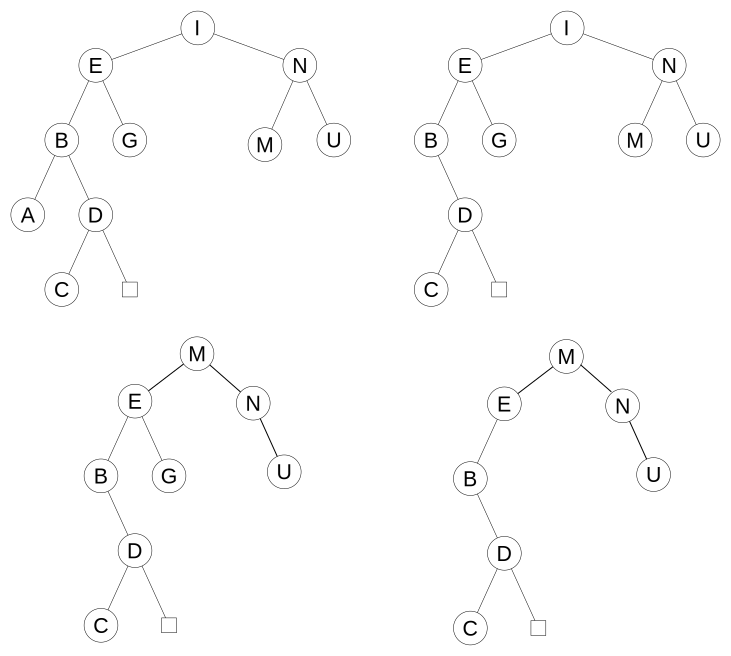
\includegraphics[width=0.8\textwidth]{avl_search_tree_delete}
      \caption{Löschen von A, I, G}
    \end{figure}
    
  \item $ $

    \begin{figure}[h!]
      \centering
      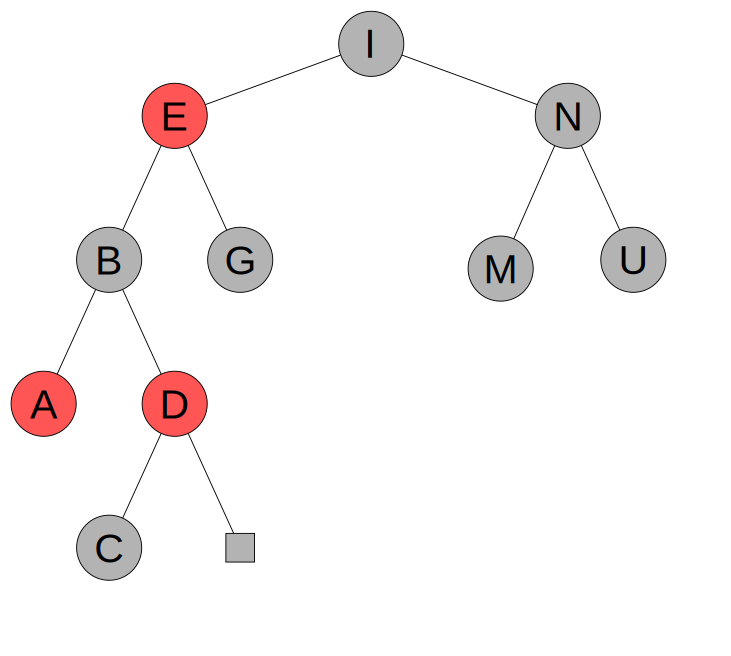
\includegraphics[width=0.4\textwidth]{avl_search_tree_red_black}
      \caption{Rot-Schwarz Version des Baumes}
    \end{figure}
    
  \item $ $

    \begin{figure}[h!]
      \centering
      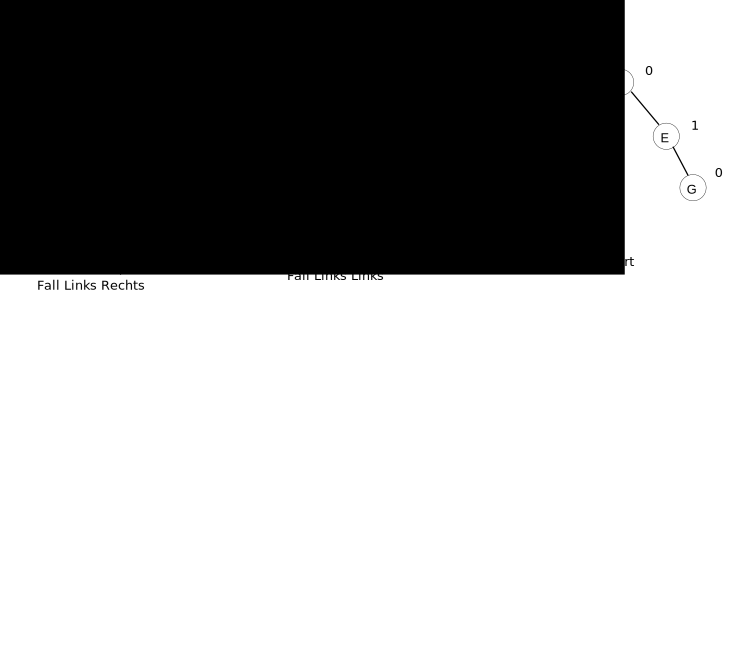
\includegraphics[width=0.8\textwidth]{avl_search_tree_rotate}
      \caption{AVL Rotationen}
    \end{figure}
    
\end{enumerate} 

\subsection*{Aufgabe 3}
\begin{enumerate}[a)]
  \item 
    Angenommen, ein schwarzer Knoten ($A$) hat ein Blatt ($B$) als Nachbarn.
    Wenn im Pfad von der Wurzel bis zum gemeinsamen Vorgänger von $A$ und $B$
    $n$ schwarze Knoten vorgekommen sind, dann kommen im Pfad von der Wurzel zu
    $B$ $n+1$ schwarze Knoten vor (da alle Blätter schwarz sind). Da $A$ kein
    Blatt ist, hat $A$ mindestens ein Blatt ($C$) als indirekten Nachfolger. Der
    Pfad dorthin beinhaltet also mindestens $n+2$ schwarze Knoten (da auch $C$
    schwarz sein muss). Dies verletzt allerdings die Eigenschaft von
    Rot-Schwarz-Bäumen, dass jeder Pfad von einem Knoten (hier der Wurzel) zu
    allen Blättern gleich lang sein muss. Im Falle von $B$ und $C$ gilt das aber
    nicht, da $n+1 \neq n+2$. Also kann ein schwarzer Knoten kein Blatt als
    Nachbarn haben.
  \item 
    Man kann einen AVL-Baum wie folgt als Prioritätswarteschlange verwenden:
    
    Jeder Prozess wird einem Knoten zugeordnet. Der Wert dieses Knotens ist die
    Zeit, die bereits für diesen Prozess aufgewendet wurde. In jedem
    Iterationsschritt wird der Prozess ausgewählt, für den am wenigsten Zeit
    aufgewendet wurde (unten links im AVL-Baum). Dieser Prozess wird nun
    ausgeführt, bis eine bestimmte Maximalzeit erreicht wird, oder der Prozess
    endet. Ist der Prozess nicht zu Ende berechnet, wird er wieder in den
    AVL-Baum eingefügt. Dieser Iterationsschritt wird sooft ausgeführt, bis alle
    Prozesse beendet sind. Durch diesen Algorithmus wird garantiert, dass
    kleinere Aufgaben schnell erledigt werden und die Arbeitszeit von größeren
    Prozessen gleichmäßig aufgeteilt wird.
    
    Die Operationen, die man dafür benötigt sind das Finden des minimalen
    Elements, das löschen dieses Elements und das Einfügen des aktualisierten
    Wertes. Alle diese Operationen haben beim AVL-Baum die Komplexität
    $\mathcal{O}(\log n)$.
    
    Man könnte diesen Algorithmus auch mit einem minHeap durchführen. Der
    gesamte Algorithmus hätte die gleiche Komplexität, da man das Minimum zwar
    in $\mathcal{O}(1)$ finden kann, aber die anderen Operationen auch in
    $\mathcal{O}(\log n)$ liegen. Allerdings ist der Nachteil des Heaps bei
    diesem Algorithmus, dass es kein größeres Element als das neu Eingefügte
    gibt. Der Grund dafür ist, dass jeder Prozess gleich viel Zeit bekommt,
    bevor ein neuer begonnen wird. Fügt man allerdings immer ein maximales
    Element unten in den Heap ein, so wird der Heap danach nicht neu sortiert.
    Nach mehrfachem Einfügen an der gleichen Stelle wird der Heap deshalb immer
    tiefer, was zu einer Verschlechterung der Laufzeit führt.
  \end{enumerate}

\end{document}
